\documentclass{beamer}

% opacity bugfix: see http://tug.org/pipermail/pdftex/2007-December/007480.html
\pdfpageattr {/Group << /S /Transparency /I true /CS /DeviceRGB>>}

\usepackage[utf8]{inputenc}
\usepackage[OT1]{fontenc}

\usepackage{tikz}
\usetikzlibrary{%
   arrows,%
   calc,%
   fit,%
   patterns,%
   plotmarks,%
   shapes.geometric,%
   shapes.misc,%
   shapes.symbols,%
   shapes.arrows,%
   shapes.callouts,%
   shapes.multipart,%
   shapes.gates.logic.US,%
   shapes.gates.logic.IEC,%
   er,%
   automata,%
   backgrounds,%
   chains,%
   topaths,%
   trees,%
   petri,%
   mindmap,%
   matrix,%
   calendar,%
   folding,%
   fadings,%
   through,%
   patterns,%
   positioning,%
   scopes,%
   decorations.fractals,%
   decorations.shapes,%
   decorations.text,%
   decorations.pathmorphing,%
   decorations.pathreplacing,%
   decorations.footprints,%
   decorations.markings,%
   shadows}
\usepackage{animate}
\usepackage{amssymb, amsmath, amsfonts, enumerate}
\usepackage{pifont}
%\usepackage{bbold}
\newcommand\hmmax{0}
\usepackage{bm}
%\usepackage{dsfont}
\usepackage{pxfonts}
\usepackage{xcolor}
\usepackage{url}

\usepackage[backend=bibtex,style=authoryear,dashed=false]{biblatex}
\addbibresource{refs.bib}
%\renewcommand{\bibfont}{\normalfont\scriptsize}
\setlength{\bibhang}{3ex}

\usepackage{hyperref}

\usetheme[official=false,department=none]{tue2008}
%\usefonttheme{default}


%\usetheme[secheader]{Boadilla}
%\setbeamercovered{transparent}
%\setbeamercovered{invisible}
%\setbeamertemplate{navigation symbols}{}
%\setbeamertemplate{bibliography item}[text] % numbered references
%\useoutertheme{infolines}
%\setbeamertemplate{headline}{}
%\setbeamertemplate{footline}{\hspace*{5mm}\hfill\insertframenumber\hspace*{5mm}\vspace{3mm}}
%\setbeamercolor{alerted text}{fg=orange!80!black}

% ------------------------------------------------------------------------------

\newcommand{\vcenterbox}[1]{\ensuremath{\vcenter{\hbox{#1}}}}
%
\newcommand{\reals}{\mathbb{R}}
\newcommand{\posreals}{\reals_{>0}}
\newcommand{\posrealszero}{\reals_{\ge 0}}
\newcommand{\naturals}{\mathbb{N}}

\newcommand{\dd}{\,\mathrm{d}}

\newcommand{\mbf}[1]{\mathbf{#1}}
\newcommand{\bs}[1]{\boldsymbol{#1}}
\renewcommand{\vec}[1]{{\bm#1}}

\newcommand{\uz}{^{(0)}} % upper zero
\newcommand{\un}{^{(n)}} % upper n
\newcommand{\ui}{^{(i)}} % upper i
\newcommand{\uell}{^{(\ell)}} % upper ell

\newcommand{\ul}[1]{\underline{#1}}
\newcommand{\ol}[1]{\overline{#1}}

\newcommand{\Rsys}{R_\text{sys}}
\newcommand{\lRsys}{\ul{R}_\text{sys}}
\newcommand{\uRsys}{\ol{R}_\text{sys}}

\newcommand{\Fsys}{F_\text{sys}}
\newcommand{\lFsys}{\ul{F}_\text{sys}}
\newcommand{\uFsys}{\ol{F}_\text{sys}}

\def\Tsys{T_\text{sys}}

\def\tmax{t_\text{max}}
\def\tnow{t_\text{now}}
\def\tpnow{t^+_\text{now}}

\newcommand{\ptk}{p^k_t}

\newcommand{\E}{\operatorname{E}}
\newcommand{\V}{\operatorname{Var}}
\newcommand{\sd}{\operatorname{sd}}

\newcommand{\wei}{\operatorname{Wei}} % Weibull Distribution
\newcommand{\ig}{\operatorname{IG}}   % Inverse Gamma Distribution
\newcommand{\ber}{\operatorname{Bernoulli}} 
\newcommand{\bin}{\operatorname{Binomial}}
\newcommand{\be}{\operatorname{Beta}} 
\newcommand{\bebin}{\operatorname{Beta-binomial}}
\newcommand{\norm}{\operatorname{N}}

\def\then{{\structure{$\rule[0.35ex]{2ex}{0.5ex}\!\!\!\blacktriangleright$}}}
\def\play{{\structure{$\blacktriangleright$}}}
\def\gplus{{\structure{\rule[0.45ex]{1.4ex}{0.4ex}\hspace{-0.9ex}\rule[0.0ex]{0.4ex}{1.3ex}\hspace{0.5ex}}}}
\def\gminus{{\structure{\rule[0.45ex]{1.4ex}{0.4ex}}}}


\def\yz{y\uz}
\def\yn{y\un}
%\def\yi{y\ui}
\newcommand{\yfun}[1]{y^{({#1})}}
\newcommand{\yfunl}[1]{\ul{y}^{({#1})}}
\newcommand{\yfunu}[1]{\ol{y}^{({#1})}}

\def\ykt{y_{k,t}}

\def\ykz{y\uz_k}
\def\ykn{y\un_k}

\def\yktz{y\uz_{k,t}}
\def\yktn{y\un_{k,t}}

\def\yzl{\ul{y}\uz}
\def\yzu{\ol{y}\uz}
\def\ynl{\ul{y}\un}
\def\ynu{\ol{y}\un}
\def\yil{\ul{y}\ui}
\def\yiu{\ol{y}\ui}

\def\ykzl{\ul{y}\uz_k}
\def\ykzu{\ol{y}\uz_k}
\def\yknl{\ul{y}\un_k}
\def\yknu{\ol{y}\un_k}

\def\yktzl{\ul{y}\uz_{k,t}}
\def\yktzu{\ol{y}\uz_{k,t}}
\def\yktnl{\ul{y}\un_{k,t}}
\def\yktnu{\ol{y}\un_{k,t}}


\def\nz{n\uz}
\def\nn{n\un}
%\def\ni{n\ui}
\newcommand{\nfun}[1]{n^{({#1})}}
\newcommand{\nfunl}[1]{\ul{n}^{({#1})}}
\newcommand{\nfunu}[1]{\ol{n}^{({#1})}}

\def\nkz{n\uz_k}
\def\nkn{n\un_k}
\newcommand{\nkzfun}[1]{n\uz_{#1}}

\def\nkt{n_{k,t}}

\def\nktz{n\uz_{k,t}}
\def\nktn{n\un_{k,t}}


\def\nzl{\ul{n}\uz}
\def\nzu{\ol{n}\uz}
\def\nnl{\ul{n}\un}
\def\nnu{\ol{n}\un}
\def\nil{\ul{n}\ui}
\def\niu{\ol{n}\ui}

\def\nkzl{\ul{n}\uz_k}
\def\nkzu{\ol{n}\uz_k}
\def\nknl{\ul{n}\un_k}
\def\nknu{\ol{n}\un_k}

\def\nktzl{\ul{n}\uz_{k,t}}
\def\nktzu{\ol{n}\uz_{k,t}}
\def\nktnl{\ul{n}\un_{k,t}}
\def\nktnu{\ol{n}\un_{k,t}}

\def\taut{\tau(\vec{t})}
\def\taux{\tau(\vec{x})}
\def\ttau{\tilde{\tau}}
\def\ttaut{\ttau(\vec{t})}
\def\ttaux{\ttau(\vec{x})}

\def\MZ{\mathcal{M}\uz}
\def\MN{\mathcal{M}\un}

\def\MkZ{\mathcal{M}\uz_k}
\def\MkN{\mathcal{M}\un_k}

\def\MktZ{\mathcal{M}\uz_{k,t}}
\def\MktN{\mathcal{M}\un_{k,t}}

\def\PZ{\Pi\uz}
\def\PN{\Pi\un}

\def\PkZ{\Pi\uz_k}
\def\PkN{\Pi\un_k}
\newcommand{\PZi}[1]{\Pi\uz_{#1}}

\def\PktZ{\Pi\uz_{k,t}}
\def\PktN{\Pi\un_{k,t}}
\newcommand{\PtZi}[1]{\Pi\uz_{#1,t}}
\newcommand{\PkZi}[1]{\Pi\uz_{k,#1}}

\newcommand{\az}{\alpha\uz}
\newcommand{\an}{\alpha\un}
\newcommand{\bz}{\beta\uz}
\newcommand{\bn}{\beta\un}


\def\blau#1{{\color{tuegreen}#1}}
\def\rot#1{{\color{tuered}#1}}
\def\gruen#1{{\color{tueblue}#1}}

\def\yzr{\rot{\yz}}
\def\ynr{\rot{\yn}}
\def\byzr{\rot{\byz}}
\def\bynr{\rot{\byn}}
\def\yzor{\rot{y\uz_1}}
\def\yzjr{\rot{y\uz_j}}
\def\yzkr{\rot{y\uz_k}}
\def\yzlr{\rot{\yzl}}
\def\yzur{\rot{\yzu}}
\def\ynjr{\rot{y\un_j}}
\def\ynlr{\rot{\ynl}}
\def\ynur{\rot{\ynu}}
\def\yzjlr#1{\rot{\ul{y}\uz_#1}}
\def\yzjur#1{\rot{\ol{y}\uz_#1}}

\def\yktzr{\rot{\yktz}}
\def\yktnr{\rot{\yktn}}

\def\nzg{\gruen{\nz}}
\def\nng{\gruen{\nn}}
\def\nzlg{\gruen{\nzl}}
\def\nzug{\gruen{\nzu}}
\def\nnlg{\gruen{\nnl}}
\def\nnug{\gruen{\nnu}}
\def\nzjlg#1{\gruen{\ul{n}\uz_#1}}
\def\nzjug#1{\gruen{\ol{n}\uz_#1}}

\def\nktzg{\gruen{\nktz}}
\def\nktng{\gruen{\nktn}}

\def\psib{\blau{\psi}}
\def\bpsib{\blau{{b}(\psi)}}


% ------------ shading start
\newsavebox{\tempbox}
\newcommand\leftrightshading[3]{%
  \begin{tikzfadingfrompicture}[name=inputtext]
    \node [text=white] {#1};
  \end{tikzfadingfrompicture}
  \begin{lrbox}{\tempbox}%
    \begin{tikzpicture}
      \node [text=white,inner sep=0pt,outer sep=0pt] (textnode) {#1};
      \shade[path fading=inputtext,fit fading=false,left color=#2,right color=#3]
      (textnode.south west) rectangle (textnode.north east);
    \end{tikzpicture}%
  \end{lrbox}
  % Now we use the fading in another picture:
  \usebox\tempbox{}%
}
% ------------ shading end


%\def\PZc{\mathrm I\!\Pi\uz}
\def\PZc{\leftrightshading{$\mathrm I\!\Pi\uz$}{blue}{red}}
\def\PktZc{\leftrightshading{${\mathrm I\!\Pi_{k,t}\uz}$}{blue}{red}}
%\def\PNc{\PN}
\def\PNc{\leftrightshading{$\mathrm I\!\Pi\un$}{blue}{red}}



\def\Eta{\mathrm{H}}
\def\EZ{\mathrm{H}\uz}
\def\EN{\mathrm{H}\un}

\newcommand{\ez}{\eta_0}
\newcommand{\eo}{\eta_1}

\def\ezl{\ul{\eta}_0}
\def\ezu{\ol{\eta}_0}

\def\ezz{\eta_0\uz}
\def\ezn{\eta_0\un}
\def\eoz{\eta_1\uz}
\def\eon{\eta_1\un}

\def\ezzl{\ul{\eta}_0\uz}
\def\ezzu{\ol{\eta}_0\uz}
\def\eznl{\ul{\eta}_0\un}
\def\ezzn{\ol{\eta}_0\un}

\def\eozl{\ul{\eta}_1\uz}
\def\eozu{\ol{\eta}_1\uz}
\def\eonl{\ul{\eta}_1\un}
\def\eonu{\ol{\eta}_1\un}

\def\eol{\ul{\eta}_1}
\def\eou{\ol{\eta}_1}

\def\czl{\ul{c}\uz}
\def\czu{\ol{c}\uz}

\def\cnl{\ul{c}\un}
\def\cnu{\ol{c}\un}

\def\ezlz{{\eta_0^l}{}^{(0)}}
\def\ezuz{{\eta_0^u}{}\uz}

\def\ezln{{\eta_0^l}{}^{(n)}}
\def\ezun{{\eta_0^u}{}\un}


\def\ezg{\gruen{\ez}}
\def\eor{\rot{\eo}}

\def\ezlg{\gruen{\ezl}}
\def\ezug{\gruen{\ezu}}

\def\ezzg{\gruen{\ezz}}
\def\ezng{\gruen{\ezn}}
\def\eozr{\rot{\eoz}}
\def\eonr{\rot{\eon}}


%%\def\blau#1{{\color{lmugreen2}#1}}
%\def\rot#1{{\color{red}#1}}
%\def\gruen#1{{\color{blue}#1}}

\newcommand{\x}{\vec{x}}

\def\tnow{t_\text{now}}
\def\tpnow{t^+_\text{now}}

\newcommand{\cmark}{{\color{tuegreen}\ding{51}}}
\newcommand{\xmark}{{\color{tuered}\ding{55}}}

\newcommand{\comp}[1]{\raisebox{-1mm}{\tikz{\node[%type1
rectangle,rounded corners=0mm,draw,fill=tuepmsgreen!70,thick,inner sep=0pt,minimum size=4mm]{#1};}}}

\newcommand{\cyansec}[1]{\textcolor{tuecyan}{\large\bf #1}}
\newcommand{\cyanalert}[1]{\textcolor{tuecyan}{#1}}
\newcommand{\bluesec}[1]{\textcolor{tueblue}{\large\bf #1}}
\newcommand{\bluealert}[1]{\textcolor{tueblue}{#1}}

\setbeamertemplate{itemize item}{\tiny\raise1.5pt\hbox{\color{tueblue}$\blacktriangleright$}}

% ------------------------------------------------------------------------------


\title{Sets of Priors\\ Reflecting Prior-Data Conflict and Agreement}

\author{\ul{Gero Walter}\inst{1}, Frank Coolen\inst{2}}
\institute{ \inst{1} Eindhoven University of Technology, Eindhoven, NL\\ 
            \inst{2} Durham University, Durham, UK \\[2ex]
            \url{g.m.walter@tue.nl} \\[2ex]
            
\includegraphics[height=9mm]{logos/tuelogo} \quad 
            
\includegraphics[height=9mm]{logos/logounidurham-large} \quad
            
\includegraphics[height=9mm]{logos/dinalog-hp} }
\date{IPMU Eindhoven 2016-06-21}

\begin{document}

\frame{
\titlepage
}

\addtocounter{framenumber}{-1} 


\begin{frame}{Bayesian Inference}
\vspace*{-2ex}
\begin{align*}
\begin{array}{ccccl}
\uncover<1->{\text{expert info}        & + & \text{data}                & \to & \text{complete picture} \\[1.5ex]}
\uncover<2->{\text{prior distribution} & + & \text{sample distribution} & \to & \text{posterior distribution} \\[1.5ex]
 f(p) & \times & f(s \mid p) & \propto & f(p \mid s) \\
 & & & & \qquad\text{\bluealert{\play\ Bayes' Rule}} \\}
%\uncover<3->{\downarrow & & \downarrow & & \hspace*{3ex} \downarrow \\
\uncover<4->{\text{Beta prior}}   & & \uncover<3->{\text{Binomial}}         & & \uncover<5->{\text{Beta posterior}} \\
\uncover<4->{}                    & & \uncover<3->{\text{distribution}}     & & \uncover<5->{\qquad \text{\bluealert{\play\ conjugacy}}}\\[1ex]
\uncover<4->{p \sim \be(\az,\bz)} & & \uncover<3->{s \mid p \sim \bin(n,p)} & & \uncover<5->{p \mid s \sim \be(\an,\bn)}
\end{array}
\end{align*}
\vspace*{-3ex}
\begin{tikzpicture}
\uncover<6->{%
\node at (0,0) {\parbox{0.99\textwidth}{%
\begin{itemize}
\item conjugate prior makes learning about parameter tractable,\\  %posterior distribution
      just update hyperparameters:\quad $\az \to \an$, $\bz \to \bn$
\item closed form for some inferences: $\E[p\mid s] = \frac{\an}{\an+\bn}$
\end{itemize}}};}
\uncover<3-5>{%
\node at (-0.5,0) {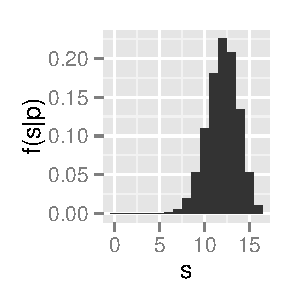
\includegraphics[width=0.25\textwidth]{figs/smallfig-binom}};}
\uncover<4-5>{%
\node at (-4.5,0) {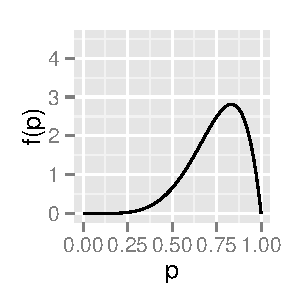
\includegraphics[width=0.25\textwidth]{figs/smallfig-prior}};}
\uncover<5>{%
\node at ( 3.5,0) {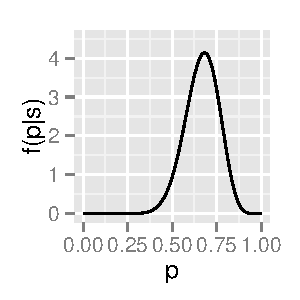
\includegraphics[width=0.25\textwidth]{figs/smallfig-posterior}};}
\end{tikzpicture}
\end{frame}


\begin{frame}{Prior-Data Conflict}

What if expert information and data tell different stories?\\
\begin{tikzpicture}
[pfeil/.style={-latex', line width=1mm, color=tuered, shorten <=1mm},
 cyanrand/.style={rounded corners, text centered, draw=tuecyan!50, inner sep=1mm, line width=0.7mm},
 redbrace/.style={draw=tuered, decoration=brace, decorate, line width=0.8mm},
 redbox/.style={text centered, draw=tuered, inner sep=1.5mm, line width=1mm, minimum width=0.75\textwidth}]
\uncover<2>{%
\node at (0,0) %
{\parbox{\textwidth}{%
\begin{block}{Prior-Data Conflict}
\begin{itemize}
\item \emph{informative prior beliefs} and \emph{trusted data}\\ %\rule{0ex}{3ex}\\
(sampling model correct, no outliers, etc.) are in conflict%\\%[2ex]
\item ``[\ldots] the prior [places] its mass primarily on distributions
in the sampling model for which the observed data is surprising''\\
\parencite{2006:evans}
\item there are not enough data to overrule the prior
\end{itemize}
\end{block}%
}};}
\uncover<3->{%
\node at (0,1.7) %
{\parbox{\textwidth}{%
\play\ reparametrisation helps to understand effect of prior-data conflict:
}};}
\uncover<4->{%
\node at (0,0.2) {\parbox[c]{\textwidth}{%
\begin{align*}
\nzg &= \az + \bz\,,
&
\yzr &= \frac{\az}{\az + \bz}\,, \quad \text{which are updated as}\\%[1.5ex]
\nng &= \nzg + n\,, 
&
\ynr &=  \frac{\nzg}{\nzg + n} \, \yzr + \frac{n}{\nzg + n} \cdot \frac{s}{n}
\end{align*}
}};}
\uncover<5->{%
\node[cyanrand] (yz) at (-0.9,-1.9) {$\yzr = \E[p]$};
\draw [pfeil] (yz.north east) to [out= 30,in=260] ( 0.9,-0.65);
\draw [pfeil] (yz.north west) to [out=130,in=240] (-1.7,0.4);}
\uncover<6->{%
\node[cyanrand] (yn) at ( 1.4,-1.9) {$\ynr = \E[p \mid s]$};
\draw [pfeil] (yn.north)      to [out=130,in=280] (-1.4,-0.65);}
\uncover<7->{%
\node[cyanrand] (ml) at ( 4.3,-1.9) {ML estimator $\hat{p}$};
\draw [pfeil] (ml.north)      to [out=100,in=330] (3.6,-0.65);}
\uncover<8->{%
\node[cyanrand] (nz) at (-4  ,-1.9) {$\nzg =$ pseudocounts};
\draw [pfeil] (nz.north)      to [out=90,in=270] (-4.0,-0.65);
\draw [pfeil] (nz.north west) to [out=95,in=240] (-5.2, 0.5);}
\uncover<9->{%
\node[redbox] at (0,-2.8) {$\E[p \mid s] = \ynr$ is a weighted average of $\E[p]$ and $\hat{p}$!};}
\uncover<10>{%
\node[redbox] at (0,-4.0) {$\V[p \mid s] = \dfrac{\ynr (1-\ynr)}{\nng + 1}$ decreases with $n$!};}
\end{tikzpicture}

\end{frame}


\begin{frame}{Prior-Data Conflict}
\tikz{\draw[fill,gray!20!white] (0,0) rectangle (0.5,0.3); \draw[tuegreen,very thick] (0,0.15) -- (0.5,0.15);} Prior $\yzr = 0.75$, $\nzg=8$
\qquad \uncover<2->{%
\tikz{\draw[fill,gray!20!white] (0,0) rectangle (0.5,0.3); \draw[tuedarkblue,very thick] (0,0.15) -- (0.5,0.15);} Posterior}
\begin{tikzpicture}
\uncover<1>{\node at (0,0) {\includegraphics[width=0.9\textwidth]{figs/betasgdens0.pdf}};}
\uncover<2>{\node at (0,0) {\includegraphics[width=0.9\textwidth]{figs/betasgdens.pdf}};}
\uncover<3>{\node at (0,0) {\includegraphics[width=0.9\textwidth]{figs/betasgpdf.pdf}};}
\uncover<2->{%
\node[fill=white] at (-2.8,1.4) {$\frac{s}{n}=\frac{12}{16}$};
\node[fill=white] at ( 3.5,1.4) {$\frac{s}{n}=\frac{0}{16}$};
}
\end{tikzpicture}
\end{frame}

\begin{frame}{Sets of Priors}
\tikz{\draw[fill,gray!20!white] (0,0) rectangle (0.5,0.3); \draw[tuegreen,very thick] (0,0.15) -- (0.5,0.15);}
Prior $\yzr \in [0.7, 0.8]$, $\nzg \in [1,8]$
\qquad \uncover<2->{%
\tikz{\draw[fill,gray!20!white] (0,0) rectangle (0.5,0.3); \draw[tuedarkblue,very thick] (0,0.15) -- (0.5,0.15);} Posterior}
\begin{tikzpicture}
\uncover<1>{\node at (0,0) {\includegraphics[width=0.9\textwidth]{figs/betaset0.pdf}};}
\uncover<2>{\node at (0,0) {\includegraphics[width=0.9\textwidth]{figs/betaset1.pdf}};}
\uncover<1->{%
\node[fill=white] at (-2.8,1.4) {$\frac{s}{n}=\frac{12}{16}$};
\node[fill=white] at ( 3.5,1.4) {$\frac{s}{n}=\frac{0}{16}$};
}
\end{tikzpicture}
\end{frame}

\iffalse
\begin{frame}{Sets of Priors}
%***change this***
%\item[\play] 
\textbf{Add \alert{imprecision} as new modelling dimension:\\
\alert{Sets of priors}\ldots}
\begin{tikzpicture}
\node at (0,0) %
{\parbox{\textwidth}{%
\begin{itemize}%[<+->]
% \begin{itemize}
 \item[] \ldots\ model uncertainty in probability statements %***show lottery A, B box
         % How is uncertainty about $\Rsys(t)$ expressed?
 \item<3->[] \ldots\ allow for partial or vague information on $\ptk$'s
         % Choosing all these Beta parameters is hard \ldots\\
 \item<4->[] \ldots\ highlight prior-data conflict.
         % see later
\end{itemize} %
\begin{itemize}
\item<5-> Separate uncertainty \emph{whithin the model} (reliability statements)\\
% ie what do we expect to see if components follow a Weibull(3.5,2) 
from uncertainty \emph{about the model} (which parameters).
\item<6-> Systematic sensitivity analysis / robust Bayesian approach
\item<7-> \textcite{2009:WalterAugustin}, \textcite{2013:diss-gw}:\\
vary $(\nzg, \yzr)$ in a set $\PZc = [\nzlg, \nzug] \times [\yzlr, \yzur]$\\
\quad\play\ easy elicitation, tractability \& prior-data conflict sensitivity
\item<8-> Bounds for inferences (point estimate, prediction, \ldots)\\
by min/max over $\PZc$ %or $\PNc$
\end{itemize}
}};
\uncover<2>{%
\node at (0,0.7) %
{\parbox{\textwidth}{%
\begin{block}{Uncertainty about probability statements}
\centerline{smaller sets $=$ more precise probability statements}
\vspace*{1ex}
\parbox[t]{0.45\textwidth}{\centering \textbf{Lottery A}\\
                          Number of winning tickets:\\
                          exactly known as 5 out of 100\\
                          \play\ $P(\text{win}) = 5/100$}
\qquad
\parbox[t]{0.45\textwidth}{\centering \textbf{Lottery B}\\
                          Number of winning tickets:\\
                          not exactly known, supposedly\\
                          between 1 and 7 out of 100\\
                          \play\ $P(\text{win}) = [1/100,\, 7/100]$}
\end{block} %
}};}
\end{tikzpicture}
%***or slide 9 from talk-lund???
%\uncover<7->{\quad\play\ min and max $\Rsys(t)$ over $\PZ$ analytical in most cases!}
%$\min_{\PZ} P\left(\Tsys > t \mid \{\nz_{k,t},\yz_{k,t},\vec{t}^k\}^{1:K}\right)$
\end{frame}
\fi

\begin{frame}{Rectangular Prior Parameter Set}
\tikz{\draw[fill,gray!20!white] (0,0) rectangle (0.5,0.3); \draw[tuegreen,very thick] (0,0.15) -- (0.5,0.15);}
Prior $\yzr \in [0.7, 0.8]$, $\nzg \in [1,8]$
\qquad
\tikz{\draw[fill,gray!20!white] (0,0) rectangle (0.5,0.3); \draw[tuedarkblue,very thick] (0,0.15) -- (0.5,0.15);} Posterior
\begin{tikzpicture}
\node at (0,0) {\includegraphics[width=0.9\textwidth]{figs/paramsets1.pdf}};
\node[fill=white] at (-3.0,0.5) {$\frac{s}{n}=\frac{12}{16}$};
\node[fill=white] at ( 1.8,0.5) {$\frac{s}{n}=\frac{0}{16}$};
\end{tikzpicture}
\parencite{2009:WalterAugustin,2013:diss-gw}
\end{frame}


\begin{frame}{Vague Prior Information}
\tikz{\draw[fill,gray!20!white] (0,0) rectangle (0.5,0.3); \draw[tuegreen,very thick] (0,0.15) -- (0.5,0.15);}
Prior $\yzr \in [0.25, 0.75]$, $\nzg \in [3,8]$
\qquad \uncover<2->{%
\tikz{\draw[fill,gray!20!white] (0,0) rectangle (0.5,0.3); \draw[tuedarkblue,very thick] (0,0.15) -- (0.5,0.15);} Posterior}
\begin{tikzpicture}
\uncover<1>{\node at (0,0) {\includegraphics[width=0.9\textwidth]{figs/betaset0-ipmu.pdf}};}
\uncover<2>{\node at (0,0) {\includegraphics[width=0.9\textwidth]{figs/betaset1-ipmu.pdf}};}
\uncover<2->{%
\node[fill=white] at (-3.3,1.65) {$\frac{s}{n}=\frac{4}{8}$};
\node[fill=white] at ( 1.5,1.65) {$\frac{s}{n}=\frac{8}{8}$};
}
\end{tikzpicture}
\end{frame}


\begin{frame}{Vague Prior Information}
\tikz{\draw[fill,gray!20!white] (0,0) rectangle (0.5,0.3); \draw[tuegreen,very thick] (0,0.15) -- (0.5,0.15);}
Prior $\yzr \in [0.25, 0.75]$, $\nzg \in [3,8]$
\qquad
\tikz{\draw[fill,gray!20!white] (0,0) rectangle (0.5,0.3); \draw[tuedarkblue,very thick] (0,0.15) -- (0.5,0.15);} Posterior
\begin{tikzpicture}
\node at (0,0) {\includegraphics[width=0.9\textwidth]{figs/paramsets1-ipmu.pdf}};
\node[fill=white] at (-3.3,1.65) {$\frac{s}{n}=\frac{4}{8}$};
\node[fill=white] at ( 1.5,1.65) {$\frac{s}{n}=\frac{8}{8}$};
\end{tikzpicture}
%\begin{align*}
%\nzg &\mapsto \nzg + n\,, &
%\yzr &\mapsto \yzr + \frac{s - n \yzr}{\nzg+n}
%\end{align*}
\pause%
\hspace*{8ex}%
$\nzg \mapsto \nzg + n$,
\qquad
$\yzr \mapsto \yzr + \dfrac{s - n \yzr}{\nzg+n}$
\end{frame}


\begin{frame}{New Parametrisation}
\textcite{2015:mik-isipta}: use parameters $(\ezzg,\eozr)$ defined as
\begin{align*}
\ezzg &= \nzg - 2\,, &
\eozr &= \nzg (\yzr - \frac{1}{2})
%\yz &= \frac{\eoz}{\ezz + 2} + \frac{1}{2}\,.
\end{align*}
Then the Bayesian update corresponds to
\begin{align*}
%\ezng &= \ezzg + n\,, &
%\eonr &= \eozr + s - \frac{n}{2}\,.
\ezzg &\mapsto \ezzg + n\,, &
\eozr &\mapsto \eozr + s - \frac{n}{2}\,.
\end{align*}
\uncover<2->{\includegraphics[width=0.9\textwidth]{figs/mikdomain.pdf}}
\end{frame}


\begin{frame}{New Parametrisation: Update}
%\vspace*{-0.5ex}
\tikz{\draw[fill,gray!20!white] (0,0) rectangle (0.5,0.3); \draw[tuegreen,very thick] (0,0.15) -- (0.5,0.15);}
Prior $\yzr \in [0.25, 0.75]$, $\nzg \in [3,8]$
\qquad \uncover<2->{%
\tikz{\draw[fill,gray!20!white] (0,0) rectangle (0.5,0.3); \draw[tuedarkblue,very thick] (0,0.15) -- (0.5,0.15);} Posterior}
\begin{tikzpicture}
\uncover<1>{\node at (0,0) {\includegraphics[width=0.9\textwidth]{figs/rectinmik0.pdf}};}
\uncover<2>{\node at (0,0) {\includegraphics[width=0.9\textwidth]{figs/rectinmik1.pdf}};}
\uncover<2->{%
\node[fill=white] at (-3.3,1.8) {$\frac{s}{n}=\frac{4}{8}$};
\node[fill=white] at ( 2.0,1.8) {$\frac{s}{n}=\frac{8}{8}$};
}
\end{tikzpicture}
\uncover<2>{%
\hspace*{10ex}$\ezzg \mapsto \ezzg + n$,\hspace*{8ex} $\eozr \mapsto \eozr + s - \dfrac{n}{2}$%
}
\end{frame}


\begin{frame}{New Parameter Set Shape: Boatshape}
\vspace*{2ex}
\tikz{\draw[fill,gray!20!white] (0,0) rectangle (0.5,0.3); \draw[tuegreen,very thick] (0,0.15) -- (0.5,0.15);}
Prior $\yzr \in [0.25, 0.75]$, $\nzg \in [3,8]$, $\rot{y_c} = 0.5$
\begin{tikzpicture}
\uncover<1->{\node at (0,0) {\includegraphics[width=0.9\textwidth]{figs/boatshape-alone.pdf}};}
\end{tikzpicture}%
\vspace*{-2ex}%
\uncover<2->{%
%\begin{align*}
%\EZ = \big\{(\ezg,\eor) \colon \ezl \le \ezg \le \ezu,\, \czl(\eta_0) \le  \eor \le \czu(\eta_0) \big\}\,,
%\text{ where}
%\end{align*}%
%\vspace*{-4ex}%
\begin{align*}
\czu(\eta_0) =  a \left( 1 - e^{-b(\eta_0 - \ezl)} \right) \text{ and }\, 
\czl(\eta_0) = -a \left( 1 - e^{-b(\eta_0 - \ezl)} \right)
\end{align*}}
%\begin{columns}
%\begin{column}{0.5\textwidth}
%\end{column}
%\begin{column}{0.5\textwidth}
%\end{column}
%\end{columns}
\end{frame}

\begin{frame}{Boatshape: Update}
\begin{tikzpicture}
\uncover<1-3>{\node at (-1,3) {\parbox{0.7\textwidth}{%
\tikz{\draw[fill,gray!20!white] (0,0) rectangle (0.5,0.3); \draw[tuegreen,very thick] (0,0.15) -- (0.5,0.15);}
Prior $\yzr \in [0.25, 0.75]$, $\nzg \in [3,8]$, $\rot{y_c} = 0.5$
}};}
\uncover<4-6>{\node at (-1,3) {\parbox{0.7\textwidth}{%
\tikz{\draw[fill,gray!20!white] (0,0) rectangle (0.5,0.3); \draw[tuegreen,very thick] (0,0.15) -- (0.5,0.15);}
Prior $\yzr \in [0.55, 0.97]$, $\nzg \in [3,8]$, $\rot{y_c} = 0.75$
}};}
\uncover<2-3,5-6>{\node at (8,3) {\parbox{0.7\textwidth}{%
\tikz{\draw[fill,gray!20!white] (0,0) rectangle (0.5,0.3); \draw[tuedarkblue,very thick] (0,0.15) -- (0.5,0.15);} Posterior
}};}
\uncover<1>{\node at (0,0) {\includegraphics[width=0.9\textwidth]{figs/boatshape-posterior-mik-ipmu0.pdf}};}
\uncover<2>{\node at (0,0) {\includegraphics[width=0.9\textwidth]{figs/boatshape-posterior-mik-ipmu1.pdf}};}
\uncover<3>{\node at (0,0) {\includegraphics[width=0.9\textwidth]{figs/boatshape-posterior-nor-ipmu1.pdf}};}
%\uncover<4>{\node at (0,0) {\includegraphics[width=0.9\textwidth]{figs/boatshape-posterior-hpd-ipmu1.pdf}};}
\uncover<4>{\node at (0,0) {\includegraphics[width=0.9\textwidth]{figs/boatshape-posterior-mik-ipmu2.pdf}};}
\uncover<5>{\node at (0,0) {\includegraphics[width=0.9\textwidth]{figs/boatshape-posterior-mik-ipmu3.pdf}};}
\uncover<6>{\node at (0,0) {\includegraphics[width=0.9\textwidth]{figs/boatshape-posterior-nor-ipmu3.pdf}};}
\uncover<2-3>{%
\node[fill=white] at (-3.3,1.6) {$\frac{s}{n}=\frac{4}{8}$};
\node[fill=white] at ( 2.0,1.6) {$\frac{s}{n}=\frac{8}{8}$};
}
\uncover<5-6>{%
\node[fill=white] at (-3.3,-1) {$\frac{s}{n}=\frac{6}{8}$};
\node[fill=white] at ( 2.0,-1) {$\frac{s}{n}=\frac{2}{8}$};
}
\end{tikzpicture}
\end{frame}

\begin{frame}{Strong Prior-Data Agreement Property}
\tikz{\draw[fill,gray!20!white] (0,0) rectangle (0.5,0.3); \draw[tuegreen,very thick] (0,0.15) -- (0.5,0.15);}
Prior $\yzr \in [0.32, 0.68]$, $\nzg \in [1,22]$, $\rot{y_c} = 0.5$ \qquad
\tikz{\draw[fill,gray!20!white] (0,0) rectangle (0.5,0.3); \draw[tuedarkblue,very thick] (0,0.15) -- (0.5,0.15);} Posterior
\begin{tikzpicture}
\uncover<1->{\node at (0,0) {\includegraphics[width=0.9\textwidth]{figs/boatshape-spda1.pdf}};}
\uncover<2->{%
\draw[very thick, red] (2.4,0.3) circle (0.75);
\node[red] at (3.6,-1.1) {\parbox{0.25\textwidth}{less imprecision\\ around $y_c$}};}
\end{tikzpicture}
\end{frame}

\begin{frame}{Summary \& Outlook}
\uncover<1->{%
\textbf{Summary:}
\begin{itemize}
\item[\play] Rectangular prior parameter sets give extra imprecision for data in conflict with the prior
\item[\play] New parametrisation with purely data-dependent update shift
\item[\play] Boatshape sets also give less imprecision for data exactly in line with the prior 
\end{itemize}}
\uncover<2->{%
\textbf{Outlook:}
\begin{itemize}
\item[\play] Elicitation via pre-posterior analysis
\item[\play] Parametrisation can be constructed for any distribution from exponential family
\item[\play] Other inference properties via tailored set shape
\end{itemize}}
\end{frame}

\nocite{2016:walter-coolen-ipmu}

\begin{frame}{References}
\renewcommand*{\bibfont}{\footnotesize}
%\begin{frame}[allowframebreaks]{References}
\printbibliography[heading=none,fontsize=\scriptsize]
\end{frame}

\end{document}
